% Created by tikzDevice version 0.12 on 2018-10-26 14:08:00
% !TEX encoding = UTF-8 Unicode
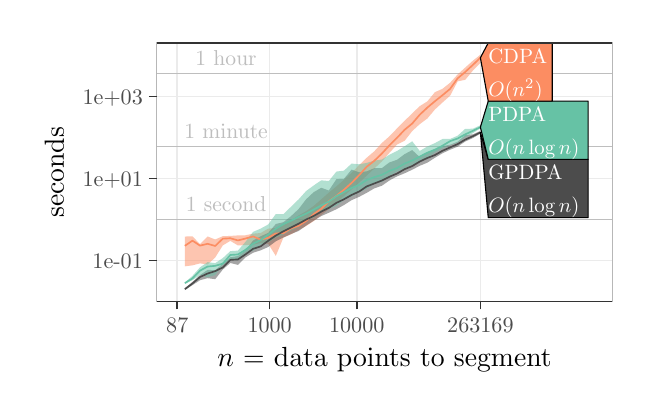
\begin{tikzpicture}[x=1pt,y=1pt]
\definecolor{fillColor}{RGB}{255,255,255}
\path[use as bounding box,fill=fillColor,fill opacity=0.00] (0,0) rectangle (216.81,130.09);
\begin{scope}
\path[clip] (  0.00,  0.00) rectangle (216.81,130.09);
\definecolor{drawColor}{RGB}{255,255,255}
\definecolor{fillColor}{RGB}{255,255,255}

\path[draw=drawColor,line width= 0.6pt,line join=round,line cap=round,fill=fillColor] ( -0.00,  0.00) rectangle (216.81,130.09);
\end{scope}
\begin{scope}
\path[clip] ( 46.58, 31.03) rectangle (211.31,124.59);
\definecolor{fillColor}{RGB}{255,255,255}

\path[fill=fillColor] ( 46.58, 31.03) rectangle (211.31,124.59);
\definecolor{drawColor}{gray}{0.92}

\path[draw=drawColor,line width= 0.6pt,line join=round] ( 46.58, 45.97) --
	(211.31, 45.97);

\path[draw=drawColor,line width= 0.6pt,line join=round] ( 46.58, 75.60) --
	(211.31, 75.60);

\path[draw=drawColor,line width= 0.6pt,line join=round] ( 46.58,105.23) --
	(211.31,105.23);

\path[draw=drawColor,line width= 0.6pt,line join=round] ( 87.44, 31.03) --
	( 87.44,124.59);

\path[draw=drawColor,line width= 0.6pt,line join=round] (118.90, 31.03) --
	(118.90,124.59);

\path[draw=drawColor,line width= 0.6pt,line join=round] ( 54.07, 31.03) --
	( 54.07,124.59);

\path[draw=drawColor,line width= 0.6pt,line join=round] (163.59, 31.03) --
	(163.59,124.59);
\definecolor{drawColor}{RGB}{190,190,190}

\path[draw=drawColor,line width= 0.6pt,line join=round] ( 46.58, 60.78) -- (211.31, 60.78);

\path[draw=drawColor,line width= 0.6pt,line join=round] ( 46.58, 87.13) -- (211.31, 87.13);

\path[draw=drawColor,line width= 0.6pt,line join=round] ( 46.58,113.47) -- (211.31,113.47);
\definecolor{fillColor}{RGB}{252,141,98}

\path[fill=fillColor,fill opacity=0.50] ( 56.81, 54.61) --
	( 59.54, 54.71) --
	( 62.28, 51.84) --
	( 65.02, 54.63) --
	( 67.76, 53.55) --
	( 70.50, 54.74) --
	( 73.23, 54.84) --
	( 75.97, 55.02) --
	( 78.71, 55.08) --
	( 81.45, 55.65) --
	( 84.19, 55.88) --
	( 86.92, 57.48) --
	( 89.66, 57.67) --
	( 92.40, 58.68) --
	( 95.14, 60.41) --
	( 97.88, 62.24) --
	(100.61, 63.80) --
	(103.35, 65.68) --
	(106.09, 68.07) --
	(108.83, 70.49) --
	(111.57, 72.76) --
	(114.30, 75.14) --
	(117.04, 77.64) --
	(119.78, 80.45) --
	(122.52, 83.09) --
	(125.26, 85.43) --
	(127.99, 88.42) --
	(130.73, 90.84) --
	(133.47, 93.69) --
	(136.21, 96.43) --
	(138.95, 99.12) --
	(141.68,101.74) --
	(144.42,103.45) --
	(147.16,106.79) --
	(149.90,107.99) --
	(152.64,110.18) --
	(155.37,113.19) --
	(158.11,115.68) --
	(160.85,118.13) --
	(163.59,120.33) --
	(163.59,117.32) --
	(160.85,114.56) --
	(158.11,111.25) --
	(155.37,110.69) --
	(152.64,105.49) --
	(149.90,103.06) --
	(147.16,100.53) --
	(144.42, 97.27) --
	(141.68, 95.24) --
	(138.95, 92.72) --
	(136.21, 89.22) --
	(133.47, 87.85) --
	(130.73, 84.88) --
	(127.99, 81.76) --
	(125.26, 79.19) --
	(122.52, 76.64) --
	(119.78, 74.06) --
	(117.04, 71.65) --
	(114.30, 69.27) --
	(111.57, 66.97) --
	(108.83, 64.53) --
	(106.09, 62.37) --
	(103.35, 60.20) --
	(100.61, 58.41) --
	( 97.88, 56.94) --
	( 95.14, 55.40) --
	( 92.40, 54.21) --
	( 89.66, 47.61) --
	( 86.92, 51.99) --
	( 84.19, 52.24) --
	( 81.45, 51.71) --
	( 78.71, 51.52) --
	( 75.97, 51.41) --
	( 73.23, 53.04) --
	( 70.50, 51.41) --
	( 67.76, 47.03) --
	( 65.02, 44.53) --
	( 62.28, 44.92) --
	( 59.54, 44.20) --
	( 56.81, 43.86) --
	cycle;
\definecolor{fillColor}{RGB}{77,77,77}

\path[fill=fillColor,fill opacity=0.50] ( 56.81, 35.93) --
	( 59.54, 38.22) --
	( 62.28, 40.69) --
	( 65.02, 42.57) --
	( 67.76, 42.46) --
	( 70.50, 44.77) --
	( 73.23, 47.14) --
	( 75.97, 47.56) --
	( 78.71, 49.64) --
	( 81.45, 53.19) --
	( 84.19, 54.71) --
	( 86.92, 55.93) --
	( 89.66, 59.14) --
	( 92.40, 59.80) --
	( 95.14, 61.97) --
	( 97.88, 64.53) --
	(100.61, 68.07) --
	(103.35, 70.65) --
	(106.09, 72.23) --
	(108.83, 71.25) --
	(111.57, 75.37) --
	(114.30, 75.48) --
	(117.04, 78.79) --
	(119.78, 77.82) --
	(122.52, 78.18) --
	(125.26, 79.32) --
	(127.99, 79.34) --
	(130.73, 81.42) --
	(133.47, 82.34) --
	(136.21, 84.39) --
	(138.95, 85.86) --
	(141.68, 83.31) --
	(144.42, 84.77) --
	(147.16, 86.11) --
	(149.90, 87.28) --
	(152.64, 87.80) --
	(155.37, 88.87) --
	(158.11, 91.27) --
	(160.85, 91.55) --
	(163.59, 92.76) --
	(163.59, 91.77) --
	(160.85, 90.20) --
	(158.11, 88.94) --
	(155.37, 87.09) --
	(152.64, 85.98) --
	(149.90, 84.71) --
	(147.16, 83.08) --
	(144.42, 81.31) --
	(141.68, 80.18) --
	(138.95, 78.76) --
	(136.21, 77.47) --
	(133.47, 76.36) --
	(130.73, 74.89) --
	(127.99, 72.97) --
	(125.26, 72.03) --
	(122.52, 70.42) --
	(119.78, 68.96) --
	(117.04, 67.76) --
	(114.30, 66.00) --
	(111.57, 64.49) --
	(108.83, 63.22) --
	(106.09, 62.02) --
	(103.35, 60.34) --
	(100.61, 58.55) --
	( 97.88, 56.61) --
	( 95.14, 55.52) --
	( 92.40, 54.26) --
	( 89.66, 52.89) --
	( 86.92, 50.83) --
	( 84.19, 49.64) --
	( 81.45, 48.75) --
	( 78.71, 47.09) --
	( 75.97, 44.37) --
	( 73.23, 45.07) --
	( 70.50, 42.68) --
	( 67.76, 39.21) --
	( 65.02, 39.57) --
	( 62.28, 38.84) --
	( 59.54, 37.05) --
	( 56.81, 35.28) --
	cycle;
\definecolor{fillColor}{RGB}{102,194,165}

\path[fill=fillColor,fill opacity=0.50] ( 56.81, 38.00) --
	( 59.54, 40.39) --
	( 62.28, 43.49) --
	( 65.02, 45.36) --
	( 67.76, 45.00) --
	( 70.50, 46.81) --
	( 73.23, 49.35) --
	( 75.97, 49.53) --
	( 78.71, 52.71) --
	( 81.45, 56.30) --
	( 84.19, 57.48) --
	( 86.92, 58.98) --
	( 89.66, 62.75) --
	( 92.40, 62.69) --
	( 95.14, 65.36) --
	( 97.88, 68.01) --
	(100.61, 71.05) --
	(103.35, 73.07) --
	(106.09, 74.92) --
	(108.83, 74.68) --
	(111.57, 78.10) --
	(114.30, 78.43) --
	(117.04, 80.98) --
	(119.78, 80.72) --
	(122.52, 81.23) --
	(125.26, 82.05) --
	(127.99, 82.44) --
	(130.73, 84.19) --
	(133.47, 85.54) --
	(136.21, 87.23) --
	(138.95, 89.03) --
	(141.68, 85.54) --
	(144.42, 87.15) --
	(147.16, 88.38) --
	(149.90, 89.86) --
	(152.64, 89.88) --
	(155.37, 91.06) --
	(158.11, 93.55) --
	(160.85, 93.57) --
	(163.59, 94.82) --
	(163.59, 93.74) --
	(160.85, 91.94) --
	(158.11, 90.58) --
	(155.37, 88.54) --
	(152.64, 87.66) --
	(149.90, 86.35) --
	(147.16, 84.96) --
	(144.42, 82.92) --
	(141.68, 81.62) --
	(138.95, 80.51) --
	(136.21, 79.11) --
	(133.47, 78.08) --
	(130.73, 76.50) --
	(127.99, 74.38) --
	(125.26, 73.62) --
	(122.52, 71.96) --
	(119.78, 70.57) --
	(117.04, 69.09) --
	(114.30, 67.82) --
	(111.57, 65.76) --
	(108.83, 64.57) --
	(106.09, 63.54) --
	(103.35, 61.56) --
	(100.61, 60.26) --
	( 97.88, 58.06) --
	( 95.14, 56.80) --
	( 92.40, 55.35) --
	( 89.66, 54.25) --
	( 86.92, 52.50) --
	( 84.19, 51.63) --
	( 81.45, 49.53) --
	( 78.71, 48.75) --
	( 75.97, 46.10) --
	( 73.23, 46.16) --
	( 70.50, 44.37) --
	( 67.76, 40.69) --
	( 65.02, 39.91) --
	( 62.28, 40.69) --
	( 59.54, 38.84) --
	( 56.81, 37.55) --
	cycle;
\definecolor{drawColor}{RGB}{252,141,98}

\path[draw=drawColor,line width= 0.6pt,line join=round] ( 56.81, 51.26) --
	( 59.54, 53.13) --
	( 62.28, 51.33) --
	( 65.02, 51.99) --
	( 67.76, 51.21) --
	( 70.50, 53.84) --
	( 73.23, 54.00) --
	( 75.97, 53.21) --
	( 78.71, 53.90) --
	( 81.45, 54.66) --
	( 84.19, 53.50) --
	( 86.92, 54.16) --
	( 89.66, 55.75) --
	( 92.40, 55.82) --
	( 95.14, 57.55) --
	( 97.88, 58.50) --
	(100.61, 60.26) --
	(103.35, 62.72) --
	(106.09, 64.62) --
	(108.83, 67.36) --
	(111.57, 69.30) --
	(114.30, 71.54) --
	(117.04, 73.99) --
	(119.78, 76.81) --
	(122.52, 79.84) --
	(125.26, 81.99) --
	(127.99, 84.61) --
	(130.73, 87.59) --
	(133.47, 90.30) --
	(136.21, 93.20) --
	(138.95, 95.45) --
	(141.68, 98.65) --
	(144.42,101.21) --
	(147.16,103.51) --
	(149.90,105.69) --
	(152.64,107.97) --
	(155.37,111.79) --
	(158.11,114.08) --
	(160.85,116.62) --
	(163.59,119.23);
\definecolor{drawColor}{gray}{0.30}

\path[draw=drawColor,line width= 0.6pt,line join=round] ( 56.81, 35.61) --
	( 59.54, 37.66) --
	( 62.28, 39.99) --
	( 65.02, 41.25) --
	( 67.76, 42.12) --
	( 70.50, 43.44) --
	( 73.23, 46.19) --
	( 75.97, 46.34) --
	( 78.71, 48.18) --
	( 81.45, 50.17) --
	( 84.19, 51.07) --
	( 86.92, 53.09) --
	( 89.66, 54.95) --
	( 92.40, 56.52) --
	( 95.14, 57.86) --
	( 97.88, 59.24) --
	(100.61, 60.75) --
	(103.35, 62.05) --
	(106.09, 63.61) --
	(108.83, 64.98) --
	(111.57, 66.80) --
	(114.30, 68.09) --
	(117.04, 69.63) --
	(119.78, 70.89) --
	(122.52, 72.73) --
	(125.26, 73.79) --
	(127.99, 74.85) --
	(130.73, 76.23) --
	(133.47, 77.38) --
	(136.21, 78.96) --
	(138.95, 80.08) --
	(141.68, 81.72) --
	(144.42, 83.01) --
	(147.16, 84.07) --
	(149.90, 85.62) --
	(152.64, 86.82) --
	(155.37, 88.02) --
	(158.11, 89.66) --
	(160.85, 90.88) --
	(163.59, 92.26);
\definecolor{drawColor}{RGB}{102,194,165}

\path[draw=drawColor,line width= 0.6pt,line join=round] ( 56.81, 37.78) --
	( 59.54, 39.48) --
	( 62.28, 42.30) --
	( 65.02, 43.77) --
	( 67.76, 44.03) --
	( 70.50, 44.81) --
	( 73.23, 47.95) --
	( 75.97, 48.13) --
	( 78.71, 49.82) --
	( 81.45, 52.04) --
	( 84.19, 53.32) --
	( 86.92, 55.27) --
	( 89.66, 57.41) --
	( 92.40, 59.10) --
	( 95.14, 60.33) --
	( 97.88, 61.69) --
	(100.61, 62.88) --
	(103.35, 64.36) --
	(106.09, 65.88) --
	(108.83, 67.23) --
	(111.57, 69.20) --
	(114.30, 70.68) --
	(117.04, 72.16) --
	(119.78, 73.28) --
	(122.52, 75.06) --
	(125.26, 76.07) --
	(127.99, 76.91) --
	(130.73, 78.33) --
	(133.47, 79.36) --
	(136.21, 80.98) --
	(138.95, 82.09) --
	(141.68, 83.51) --
	(144.42, 84.91) --
	(147.16, 86.01) --
	(149.90, 87.44) --
	(152.64, 89.09) --
	(155.37, 90.04) --
	(158.11, 91.54) --
	(160.85, 92.81) --
	(163.59, 94.14);
\definecolor{drawColor}{RGB}{190,190,190}

\node[text=drawColor,anchor=base,inner sep=0pt, outer sep=0pt, scale=  0.78] at ( 71.70, 63.71) {1 second};

\node[text=drawColor,anchor=base,inner sep=0pt, outer sep=0pt, scale=  0.78] at ( 71.70, 90.05) {1 minute};

\node[text=drawColor,anchor=base,inner sep=0pt, outer sep=0pt, scale=  0.78] at ( 71.70,116.39) {1 hour};
\end{scope}
\begin{scope}
\path[clip] ( 46.58, 31.03) rectangle (211.31,124.59);
\definecolor{drawColor}{RGB}{0,0,0}
\definecolor{fillColor}{gray}{0.30}

\path[draw=drawColor,line width= 0.4pt,line join=round,line cap=round,fill=fillColor] (163.59, 92.26) --
	(166.43, 82.50) --
	(202.52, 82.50) --
	(202.52, 61.46) --
	(166.43, 61.46) --
	cycle;
\definecolor{fillColor}{RGB}{102,194,165}

\path[draw=drawColor,line width= 0.4pt,line join=round,line cap=round,fill=fillColor] (163.59, 94.14) --
	(166.43,103.54) --
	(202.52,103.54) --
	(202.52, 82.50) --
	(166.43, 82.50) --
	cycle;
\definecolor{fillColor}{RGB}{252,141,98}

\path[draw=drawColor,line width= 0.4pt,line join=round,line cap=round,fill=fillColor] (163.59,119.23) --
	(166.43,124.59) --
	(189.56,124.59) --
	(189.56,103.54) --
	(166.43,103.54) --
	cycle;
\definecolor{drawColor}{RGB}{255,255,255}

\node[text=drawColor,anchor=base west,inner sep=0pt, outer sep=0pt, scale=  0.75] at (166.43, 75.09) {GPDPA};

\node[text=drawColor,anchor=base west,inner sep=0pt, outer sep=0pt, scale=  0.75] at (166.43, 63.21) {$O(n \log n)$};

\node[text=drawColor,anchor=base west,inner sep=0pt, outer sep=0pt, scale=  0.75] at (166.43, 96.13) {PDPA};

\node[text=drawColor,anchor=base west,inner sep=0pt, outer sep=0pt, scale=  0.75] at (166.43, 84.25) {$O(n \log n)$};

\node[text=drawColor,anchor=base west,inner sep=0pt, outer sep=0pt, scale=  0.75] at (166.43,117.18) {CDPA};

\node[text=drawColor,anchor=base west,inner sep=0pt, outer sep=0pt, scale=  0.75] at (166.43,105.30) {$O(n^2)$};
\definecolor{drawColor}{gray}{0.20}

\path[draw=drawColor,line width= 0.6pt,line join=round,line cap=round] ( 46.58, 31.03) rectangle (211.31,124.59);
\end{scope}
\begin{scope}
\path[clip] (  0.00,  0.00) rectangle (216.81,130.09);
\definecolor{drawColor}{gray}{0.30}

\node[text=drawColor,anchor=base east,inner sep=0pt, outer sep=0pt, scale=  0.80] at ( 41.63, 42.95) {1e-01};

\node[text=drawColor,anchor=base east,inner sep=0pt, outer sep=0pt, scale=  0.80] at ( 41.63, 72.58) {1e+01};

\node[text=drawColor,anchor=base east,inner sep=0pt, outer sep=0pt, scale=  0.80] at ( 41.63,102.21) {1e+03};
\end{scope}
\begin{scope}
\path[clip] (  0.00,  0.00) rectangle (216.81,130.09);
\definecolor{drawColor}{gray}{0.20}

\path[draw=drawColor,line width= 0.6pt,line join=round] ( 43.83, 45.97) --
	( 46.58, 45.97);

\path[draw=drawColor,line width= 0.6pt,line join=round] ( 43.83, 75.60) --
	( 46.58, 75.60);

\path[draw=drawColor,line width= 0.6pt,line join=round] ( 43.83,105.23) --
	( 46.58,105.23);
\end{scope}
\begin{scope}
\path[clip] (  0.00,  0.00) rectangle (216.81,130.09);
\definecolor{drawColor}{gray}{0.20}

\path[draw=drawColor,line width= 0.6pt,line join=round] ( 87.44, 28.28) --
	( 87.44, 31.03);

\path[draw=drawColor,line width= 0.6pt,line join=round] (118.90, 28.28) --
	(118.90, 31.03);

\path[draw=drawColor,line width= 0.6pt,line join=round] ( 54.07, 28.28) --
	( 54.07, 31.03);

\path[draw=drawColor,line width= 0.6pt,line join=round] (163.59, 28.28) --
	(163.59, 31.03);
\end{scope}
\begin{scope}
\path[clip] (  0.00,  0.00) rectangle (216.81,130.09);
\definecolor{drawColor}{gray}{0.30}

\node[text=drawColor,anchor=base,inner sep=0pt, outer sep=0pt, scale=  0.80] at ( 87.44, 20.05) {1000};

\node[text=drawColor,anchor=base,inner sep=0pt, outer sep=0pt, scale=  0.80] at (118.90, 20.05) {10000};

\node[text=drawColor,anchor=base,inner sep=0pt, outer sep=0pt, scale=  0.80] at ( 54.07, 20.05) {87};

\node[text=drawColor,anchor=base,inner sep=0pt, outer sep=0pt, scale=  0.80] at (163.59, 20.05) {263169};
\end{scope}
\begin{scope}
\path[clip] (  0.00,  0.00) rectangle (216.81,130.09);
\definecolor{drawColor}{RGB}{0,0,0}

\node[text=drawColor,anchor=base,inner sep=0pt, outer sep=0pt, scale=  1.00] at (128.95,  7.63) {$n$ = data points to segment};
\end{scope}
\begin{scope}
\path[clip] (  0.00,  0.00) rectangle (216.81,130.09);
\definecolor{drawColor}{RGB}{0,0,0}

\node[text=drawColor,rotate= 90.00,anchor=base,inner sep=0pt, outer sep=0pt, scale=  1.00] at ( 13.04, 77.81) {seconds};
\end{scope}
\end{tikzpicture}
